% THIS IS AN EXAMPLE DOCUMENT FOR VLDB 2012
% based on ACM SIGPROC-SP.TEX VERSION 2.7
% Modified by  Gerald Weber <gerald@cs.auckland.ac.nz>
% Removed the requirement to include *bbl file in here. (AhmetSacan, Sep2012)
% Fixed the equation on page 3 to prevent line overflow. (AhmetSacan, Sep2012)



\documentclass[sigconf, nonacm]{acmart}

%% The following content must be adapted for the final version
% paper-specific
\newcommand\vldbdoi{XX.XX/XXX.XX}
\newcommand\vldbpages{XXX-XXX}
% issue-specific
\newcommand\vldbvolume{14}
\newcommand\vldbissue{1}
\newcommand\vldbyear{2020}
% should be fine as it is
\newcommand\vldbauthors{\authors}
\newcommand\vldbtitle{\shorttitle} 
% leave empty if no availability url should be set
\newcommand\vldbavailabilityurl{URL_TO_YOUR_ARTIFACTS}
% whether page numbers should be shown or not, use 'plain' for review versions, 'empty' for camera ready
\newcommand\vldbpagestyle{plain} 

% \documentclass{vldb}
% \renewcommand{\baselinestretch}{0.99}
\usepackage{graphicx}
\usepackage{wrapfig}
\usepackage{balance}  % for  \balance command ON LAST PAGE  (only there!)
\usepackage{enumitem}
\usepackage{hyperref, xcolor}
\hypersetup{colorlinks, citecolor=blue}
     %colorlinks=false,
      %citecolor=Violet,
       %linkcolor=Red,
        %urlcolor=Blue}

\usepackage[T1]{fontenc}
\usepackage[utf8]{inputenc}
\usepackage{multirow}
\usepackage{bbding}
\usepackage{pifont}
\usepackage{wasysym}
\let\Bbbk\relax
\usepackage{amssymb}
\usepackage{array,multirow}
\usepackage{booktabs}
\usepackage{cleveref}
\usepackage{soul}
\usepackage{tikz}
\usetikzlibrary{arrows.meta,positioning,calc,decorations.pathreplacing,shapes.geometric}
\newcommand{\cstep}[1]{\tikz[baseline=-0.5ex]{\node[circle,fill=black!70,text=white,inner sep=0pt,minimum size=8pt,font=\fontsize{5.5}{6}\selectfont\bfseries]{#1};}}

% \crefformat{section}{\S#2#1#3} % see manual of cleveref, section 8.2.1
% \crefformat{subsection}{\S#2#1#3}
% \crefformat{subsubsection}{\S#2#1#3}

\usepackage{url}
\usepackage{algorithm}
% \usepackage{balance}

% \newcommand\longvar[1]{\mathchardef\UrlBreakPenalty=100
% 	\mathchardef\UrlBigBreakPenalty=100\url{#1}}

% \makeatletter
% \newcommand{\printfnsymbol}[1]{%
%   \textsuperscript{\@fnsymbol{#1}}%
% }
% \makeatother

\newcommand{\yacov}[1]{\textcolor{blue}{$\ll${Yacov: #1}$\gg$}}


% allow slight stretch to avoid overfull hboxes without full \sloppy
\emergencystretch=1em

\begin{document}

% ****************** TITLE ****************************************

\title{Enabling Data Privacy in Blockchain}
% \author[1]{} %\thanks{contributed equally} } 
% \author[1]{} %\printfnsymbol{1}}
% \author[1]{} % \printfnsymbol{1}}
% \author[2]{}
% \author[1]{}
% \affil[ ]{}
% \affil[ ]{}
% \author{
% 	Senthil Nathan, Chander Govindarajan, Adarsh Saraf, Manish Sethi, Praveen Jayachandran\\
% 	\affaddr{IBM Research}
% }
% possible, but not really needed or used for PVLDB:
%\subtitle{[Extended Abstract]
%\titlenote{A full version of this paper is available as\textit{Author's Guide to Preparing ACM SIG Proceedings Using \LaTeX$2_\epsilon$\ and BibTeX} at \texttt{www.acm.org/eaddress.htm}}}

% ****************** AUTHORS **************************************

% You need the command \numberofauthors to handle the 'placement
% and alignment' of the authors beneath the title.
%
% For aesthetic reasons, we recommend 'three authors at a time'
% i.e. three 'name/affiliation blocks' be placed beneath the title.
%
% NOTE: You are NOT restricted in how many 'rows' of
% "name/affiliations" may appear. We just ask that you restrict
% the number of 'columns' to three.
%
% Because of the available 'opening page real-estate'
% we ask you to refrain from putting more than six authors
% (two rows with three columns) beneath the article title.
% More than six makes the first-page appear very cluttered indeed.
%
% Use the \alignauthor commands to handle the names
% and affiliations for an 'aesthetic maximum' of six authors.
% Add names, affiliations, addresses for
% the seventh etc. author(s) as the argument for the
% \additionalauthors command.
% These 'additional authors' will be output/set for you
% without further effort on your part as the last section in
% the body of your article BEFORE References or any Appendices.

%\numberofauthors{4} %  in this sample file, there are a *total*
% of EIGHT authors. SIX appear on the 'first-page' (for formatting
% reasons) and the remaining two appear in the \additionalauthors section.

%\author{
% You can go ahead and credit any number of authors here,
% e.g. one 'row of three' or two rows (consisting of one row of three
% and a second row of one, two or three).
%
% The command \alignauthor (no curly braces needed) should
% precede each author name, affiliation/snail-mail address and
% e-mail address. Additionally, tag each line of
% affiliation/address with \affaddr, and tag the
% e-mail address with \email.
%
% 1st. author
%\alignauthor
%
%Ben Trovato\titlenote{Dr.~Trovato insisted his name be first.}\\
%       \affaddr{Institute for Clarity in Documentation}\\
%       \affaddr{1932 Wallamaloo Lane}\\
%       \affaddr{Wallamaloo, New Zealand}\\
%       \email{trovato@corporation.com}
%% 2nd. author
%\alignauthor
%G.K.M. Tobin\titlenote{The secretary disavows
%any knowledge of this author's actions.}\\
%       \affaddr{Institute for Clarity in Documentation}\\
%       \affaddr{P.O. Box 1212}\\
%       \affaddr{Dublin, Ohio 43017-6221}\\
%       \email{webmaster@marysville-ohio.com}
% 3rd. author
%\alignauthor Lars Th{\Large{\sf{\o}}}rv{$\ddot{\mbox{a}}$}ld\titlenote{This author is the
%one who did all the really hard work.}\\
%       \affaddr{The Th{\large{\sf{\o}}}rv{$\ddot{\mbox{a}}$}ld Group}\\
%       \affaddr{1 Th{\large{\sf{\o}}}rv{$\ddot{\mbox{a}}$}ld Circle}\\
%       \affaddr{Hekla, Iceland}\\
%       \email{larst@affiliation.org}
%\and  % use '\and' if you need 'another row' of author names
%% 4th. author
%\alignauthor Lawrence P. Leipuner\\
%       \affaddr{Brookhaven Laboratories}\\
%       \affaddr{Brookhaven National Lab}\\
%       \affaddr{P.O. Box 5000}\\

%       \email{lleipuner@researchlabs.org}
% There's nothing stopping you putting the seventh, eighth, etc.
% author on the opening page (as the 'third row') but we ask,
% for aesthetic reasons that you place these 'additional authors'
% in the \additional authors block, viz.
% Just remember to make sure that the TOTAL number of authors
% is the number that will appear on the first page PLUS the
% number that will appear in the \additionalauthors section.
%}

\author{Senthilnathan Natarajan, Manish Sethi, Dave Enyeart, Yacov Manevich, Artem Barger}
\affiliation{\institution{IBM Research}}

% \author{Manish Sethi}
% \affiliation{\institution{IBM Research}}
%
% \author{Dave Enyeart}
% \affiliation{\institution{IBM Research}}
%
% \author{Yacov Manevich}
% \affiliation{\institution{IBM Research}}
%
% \author{Artem Barger}
% \affiliation{\institution{IBM Research}}
\thanks{Yacov Manevich is now at Ava Labs. Artem Barger is now at Modelyo.}


\begin{abstract}
	some text \ldots
\end{abstract}


\maketitle

%%% do not modify the following VLDB block %%
%%% VLDB block start %%%
\pagestyle{\vldbpagestyle}
\begingroup\small\noindent\raggedright\textbf{PVLDB Reference Format:}\\
\vldbauthors. \vldbtitle. PVLDB, \vldbvolume(\vldbissue): \vldbpages, \vldbyear.\\
\href{https://doi.org/\vldbdoi}{doi:\vldbdoi}
\endgroup
\begingroup
\renewcommand\thefootnote{}\footnote{\noindent
This work is licensed under the Creative Commons BY-NC-ND 4.0 International License. Visit \url{https://creativecommons.org/licenses/by-nc-nd/4.0/} to view a copy of this license. For any use beyond those covered by this license, obtain permission by emailing \href{mailto:info@vldb.org}{info@vldb.org}. Copyright is held by the owner/author(s). Publication rights licensed to the VLDB Endowment. \\
\raggedright Proceedings of the VLDB Endowment, Vol. \vldbvolume, No. \vldbissue\ %
ISSN 2150-8097. \\
\href{https://doi.org/\vldbdoi}{doi:\vldbdoi} \\
}\addtocounter{footnote}{-1}\endgroup
%%% VLDB block end %%%

%%% do not modify the following VLDB block %%
%%% VLDB block start %%%
\ifdefempty{\vldbavailabilityurl}{}{
% \begingroup\small\noindent\raggedright\textbf{PVLDB Artifact Availability:}\\
% The source code, data, and/or other artifacts have been made available at \url{\vldbavailabilityurl}.
% \endgroup
}
%%% VLDB block end %%%

\section{Introduction}
Enterprise blockchain networks are redefining how organizations collaborate on shared data without a central intermediary. In food safety, Walmart demonstrated that a blockchain-based traceability system can reduce the time to trace contaminated produce from seven days to 2.2 seconds~\cite{7-to-2, walmart-hf}. In pharmaceuticals, the MediLedger network~\cite{mediledger} enables drug provenance tracking under the U.S. Drug Supply Chain Security Act, validated through an FDA pilot program. In global trade, GSBN~\cite{gsbn} coordinates private shipping documents across dozens of carriers and ports. In mining, MineHub~\cite{minehub} orchestrates supply-chain workflows across thousands of companies. The common foundation underlying these deployments is a permissioned blockchain: a decentralized, immutable, and transparent ledger that establishes trust among mutually distrusting parties without requiring a central authority.

Yet this very transparency creates a fundamental tension. Enterprise data is inherently private---pricing agreements between a manufacturer and supplier, patient medical records governed by HIPAA~\cite{hipaa-privacy}, identity credentials protected under GDPR~\cite{gdpr}. Storing such data on a fully replicated ledger exposes it to every network participant, including direct competitors. The consequence is stark: organizations must either accept unacceptable privacy violations, or keep private data in siloed off-chain systems, sacrificing the consistency, auditability, and trust guarantees that motivated the blockchain in the first place. This privacy-transparency tradeoff is widely recognized as one of the primary barriers to enterprise blockchain adoption.

Existing approaches are either too coarse-grained, too expensive, or too fragile. \textit{Channels}~\cite{hf}---essentially private sub-networks---provide isolation but require a separate ledger, consensus, and management for each data-sharing relationship, an operational burden that scales poorly as the number of bilateral relationships grows. \textit{Zero-knowledge proofs}~\cite{inproceedings, 7546538} offer strong cryptographic privacy but impose seconds-per-proof computational costs that are prohibitive for high-throughput enterprise workloads. \textit{Trusted Execution Environments}~\cite{ekiden, ccf} rely on specialized hardware and carry well-documented side-channel vulnerabilities. Off-chain databases coupled with on-chain hashes break transactional atomicity: a shipment record and its private invoice cannot be committed atomically across a blockchain and an external store without fragile two-phase commit protocols. None of these approaches simultaneously achieve fine-grained privacy, transactional atomicity, smart-contract integration, and low overhead without specialized hardware (Table~\ref{table:comparison}).
\begin{table}[h]
\centering
\small
\caption{Comparison of Privacy Mechanisms}
\label{table:comparison}
\begin{tabular}{|l|c|c|c|c|}
\hline
\textbf{Mechanism} & \textbf{Fine} & \textbf{Atomic} & \textbf{SC} & \textbf{No HW} \\
 & \textbf{Grained} & & \textbf{Access} & \textbf{Dep.} \\ \hline
Channels & $\times$ & $\checkmark$ & $\checkmark$ & $\checkmark$ \\ \hline
Off-chain DB & $\checkmark$ & $\times$ & $\times$ & $\checkmark$ \\ \hline
ZKPs & $\checkmark$ & $\checkmark$ & Limited\footnotemark & $\checkmark$ \\ \hline
TEEs (e.g., SGX) & $\checkmark$ & $\checkmark$ & $\checkmark$ & $\times$ \\ \hline
\textbf{Pvt. Collections} & $\checkmark$ & $\checkmark$ & $\checkmark$ & $\checkmark$ \\ \hline
\end{tabular}
\vspace{-.3cm}
\end{table}
\footnotetext{ZKP-based smart contracts require expressing all business logic as arithmetic circuits or constraint systems, which limits expressiveness compared to general-purpose languages and imposes significant per-proof computational cost (seconds per proof).}

This paper presents \textit{private data collections} (PDCs), a mechanism that enables fine-grained data privacy within a single blockchain ledger. The key insight is that by storing only the cryptographic hash of private data on the replicated ledger while confining actual data to authorized nodes, the entire network can verify the serializability and integrity of private transactions \textit{without ever seeing the private data itself}---a property we call \textit{blind validation}. Authorized peers process private data in plaintext and simultaneously record its hash on the public ledger; at commit time, any node can validate conflicts by comparing hash versions alone, with no access to the underlying private data required. This eliminates the need for expensive cryptographic primitives or specialized hardware. Unlike channels, PDCs operate within a single ledger; unlike ZKP-based approaches, they impose minimal computational overhead; and unlike off-chain stores, they guarantee transactional atomicity across public and private state. However, because private data is excluded from the consensus-driven block delivery, a critical challenge remains: ensuring that all authorized nodes obtain the private data they need before committing a block. We address this with a gossip-based protocol that proactively disseminates private data during transaction simulation and reactively retrieves missing data before commit, tolerating network partitions and dynamic membership changes.

The main contributions of this paper are as follows:
\begin{itemize}[topsep=0pt,noitemsep,leftmargin=15pt]
    \item We formalize the private data collection abstraction, identify seven design requirements (atomicity, hash-data integrity, smart-contract access control, authorized execution, dynamic membership, data lifecycle management, and data availability), and show that the \textit{execute-order-validate-commit} replication protocol is uniquely suited to support them (\S\ref{pdc}).
    \item We design a dual-layered storage architecture with a \textit{blind validation} mechanism and formally prove that on-chain hashes serve as a conflict-complete proxy for private state, enabling network-wide serializability verification without exposing private data (\S\ref{s:design}).
    \item We propose a two-phase gossip-based protocol combining proactive dissemination with reactive retrieval, supporting dynamic membership changes and tolerating network partitions (\S\ref{s:gossip}).
    \item We implement private data collections in Hyperledger Fabric, an open-source permissioned blockchain platform. The feature has been merged into the Fabric codebase (production-ready since v1.2, with continued enhancements through v2.5) and is deployed in production by organizations including Walmart, MineHub, GSBN, MediLedger, Honeywell, and Oracle.
\end{itemize}

The remainder of this paper is organized as follows. Section~2 motivates the need for data privacy through real-world use cases. Section~3 presents the core idea of our proposed mechanism and analyzes the suitability of different blockchain replication protocols. Section~4 details the design of private data transaction processing. Section~5 describes the data dissemination and retrieval protocol. Section~6 presents the threat model and security analysis. Section~7 discusses implementation. Section~8 presents a performance evaluation. Section~9 describes real-world adoption and impact. Section~10 discusses related work, and Section~11 concludes.


\section{Motivation for Ledger and Gossip}
some text \ldots

\subsection{Ledger}
some text \ldots

\par
\textbf{Public Ledger} some text \ldots

\par
\textbf{Private Ledger} some text \ldots

\par
\textbf{Channels} some text \ldots

\par
\textbf{Pluggable Database Layer} some text \ldots

\par
\subsection{Gossip}
some text \ldots



\section{Proposing Private Data Collections For Data Privacy}
\label{pdc}
\textbf{Key Idea.}
To hide the private data from specific members in a blockchain
network, we propose the following:
\begin{enumerate}[topsep=0pt,noitemsep,leftmargin=15pt]
    \item Share and store private data only on a node owned by the member
        who should see the data. To achieve this, we introduce private data
        \textit{collection} with membership. Any data intended for a
        \textit{collection} is stored only on that collection's members' node.
    \item Share and store the hash of private data on all nodes as evidence
        for tamper detection. In other words, store the hash of private data
        (present in each \textit{collection}) on the replicated ledger,
        visible to all members.
\end{enumerate}
% to share the private data only with the members
% who should see it and store the hash of private data on the replicated
% ledger as evidence for tamper detection. To achieve this, we propose
% private data collection with membership---any data stored on a collection is
% visible and reside only on the collection members' node. The hash of
% the private data and any public data get stored on the replicated ledger,
% which is visible to all nodes.
\par
Figure~\ref{fig:fsc-pvt-data-food-traceability} showcases the use of private data collection
to achieve data privacy in the food traceability use-case.
There are five private data collections, where four of them have two members, and the
rest with just one member.
%There are four private data collections, each with two members and one private data
% collection with just one member.
The replicated ledger contains public data such the order IDs, product \& lot IDs, participants
involved in each transaction, and the hash of each private data stored in each collection. For each
order ID, the respective private data such as the order details, invoices, and payment are stored
in a collection depending on who issued the order to whom. Thus, the food traceability solution
achieves data privacy.
\par
Figure~\ref{fig:fsc-pvt-data-health-care} showcases the use of private
data collection to achieve data privacy in the health-care use-case.
There are five private data collections, each with only one member.
A hospital stores its patient's medical record on a collection where the
respective hospital's node is a member.
On an as-needed basis, such as during an insurance claim, a patient can copy
their medical record located at one hospital's collection to another where the
insurance provider is a member. As the medical record evidence (i.e., the record's hash)
is present in the replicated ledger, the receiving party can ensure its authenticity.
Similarly, a patient can copy or move their medical record from one hospital's
collection to another.
% Here, each
% hospital, regulator, and insurance provider owns a private data collection.
% A patient's medical record at one hospital's collection can be copied to another
% collection in which the regulator or insurance provider is a member on an as-needed
% basis. As the medical record evidence, i.e., hash of the record, is present in the
% replicated ledger, the receiving party can ensure the record's authenticity.
% Similarly, a patient's medical record can be copied or moved from one hospital's
% collection to another when the patient shifts.
\par
\textbf{Design Requirements.}
The following requirements should be satisfied with our design to allow a wide variety of use-cases,
including the three use-cases described in \S\ref{motivation}.
\begin{enumerate}[topsep=0pt,noitemsep,leftmargin=15pt]
        \item[\textbf{R1}] As part of the transaction, a client could include a list of collection
            and private data to be stored, accessed, or modified in each collection. A submitted
            transaction should be executed only by a smart-contract hosted on nodes running in a
            blockchain network to ensure the standard data format needed to share data across different
            members and follow the agreed business processes. In other words, only a smart-contract
            can store, access, or modify a private data stored in a collection.
            % As a part of transaction, the client
            % should be able to include the name of collections and private data to be stored, accessed
            % or modified in each of that collection. The transaction submitted to a blockchain network should
            % be executed only by a smart-contract to ensure the standard data format needed for sharing data
            % across different members and following the agreed business processes. In other words, only
            % a smart-contract can store, access, or modify a data stored in a collection.
		% \item[\textbf{R1}] The private data stored on a collection must be accessed or modified
            % through a smart-contract only. The smart-contract ensures the standard data format
            % needed for sharing data across different members and following the agreed business processes.
            % The private data stored on a collection must be accessed or modified through
            % a smart-contract only. The smart-contract helps to ensure common data
            % format needed for sharing data across different members and to follow the agreed business processes.
        \item[\textbf{R2}] A transaction should be executed only on members' node with whom the private data
            is shared. In other words, a smart-contract executing a transaction should have access to all collections
            specified in the transaction and the public data stored on the replicated ledger. Hence,
            a transaction should be allowed to execute only on a subset of nodes in a network because
            a node has access to a collection only if it is a member of that collection.
            % A smart-contract, hosted on nodes running in
            % a blockchain network, that executing the transaction should be able to access all collections
        % specified in the transaction input and the public data stored on the replicated ledger.
        % As a result, the transaction may not be submitted/executed on all members' node because
        % a node can access a collection only if it is a member of that collection.
            % A transaction input needs to include the name of private data collection and
            % private data to be stored or modified. The smart-contract hosted on a blockchain network
            % that processing the transaction should be able to access all private data collections specified
            % in the transaction input as well as the public data stored on the replicated ledger.
            % As a result, the transaction may not be submitted/executed on all nodes in the network.
		\item[\textbf{R3}] When a transaction, executed by smart-contract, modifies both the public and private data,
				the atomicity and serializable isolation should be guaranteed.
		\item[\textbf{R4}] The private data's hash stored on the replicated ledger should always be in sync with the
				actual private data stored in the collection.
		\item[\textbf{R5}] The members of a collection should be mutable, i.e., a new member can be added, or an
            old member can be removed. A newly added member’s node should receive and store all private data in
            that collection, including the existing data. A removed member’s node should have access only to data
            that was persisted when it was a member.
            % The members of a collection should be mutable, i.e., a new member can be added, or an old member can be
            % removed. A newly added member's node should receive and store all private data in that collection
            % including the existing data. A removed member's node should have access only to data that
            % was persisted when it was a member.
		\item[\textbf{R6}] The data stored in a collection can have a time-to-live property.
\end{enumerate}
\begin{figure}
    \begin{center}
	    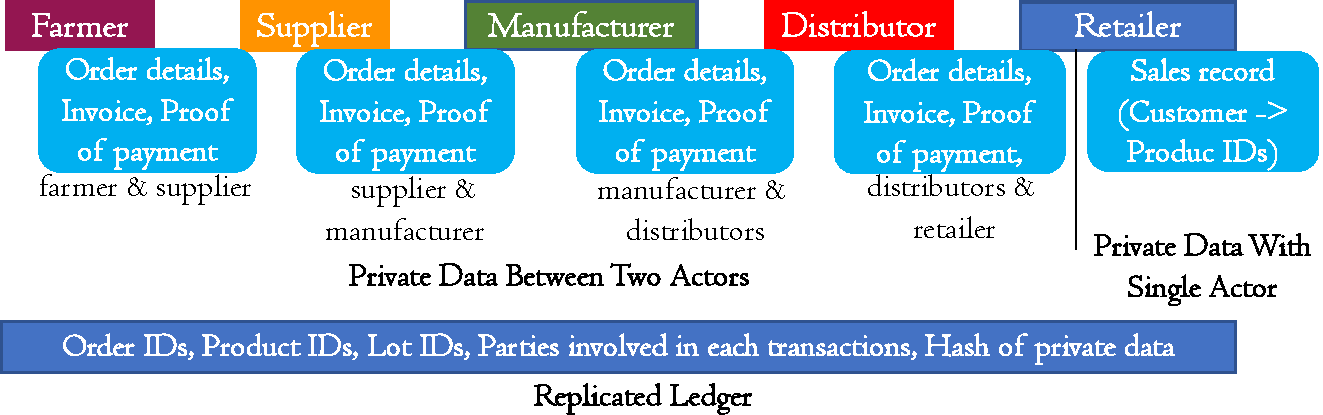
\includegraphics[scale=0.42]{fig/fsc-private-data.pdf}
  		\vspace{-.4cm}
		\caption{\small{The private/sensitive data is visible only to the appropriate parties and the proof of data existance is stored
						in a replicated ledger along with necessary information needed to enable traceability}.}
		\label{fig:fsc-pvt-data-food-traceability}
 \end{center}
  \vspace{-.5cm}
\end{figure}

\begin{figure}
    \begin{center}
			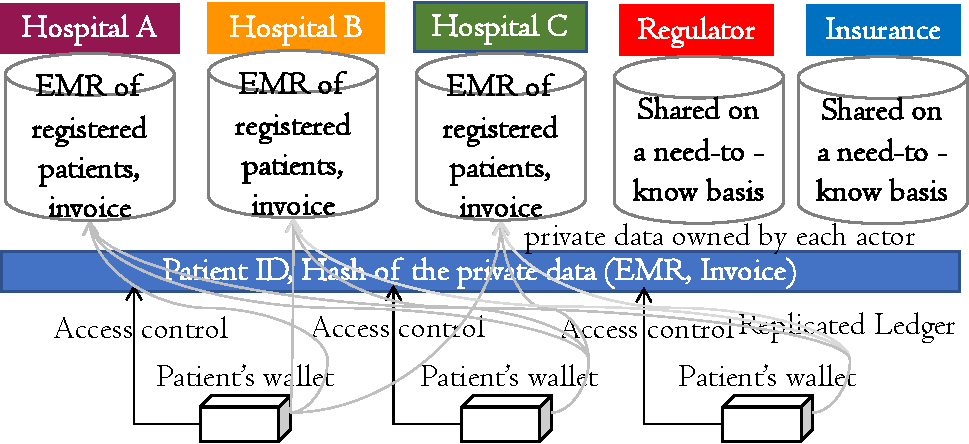
\includegraphics[scale=0.42]{fig/health-care-private-data.pdf}
  		\vspace{-.4cm}
		\caption{\small{The private/sensitive data is maintained at the node of each individual hospital's node and the proof of data
						existance is stored in a replicated ledger along with necessary information needed to share data on a need-to-know basis}.}
		\label{fig:fsc-pvt-data-health-care}
 \end{center}
  \vspace{-.5cm}
\end{figure}
\begin{figure*}
    \begin{center}
	    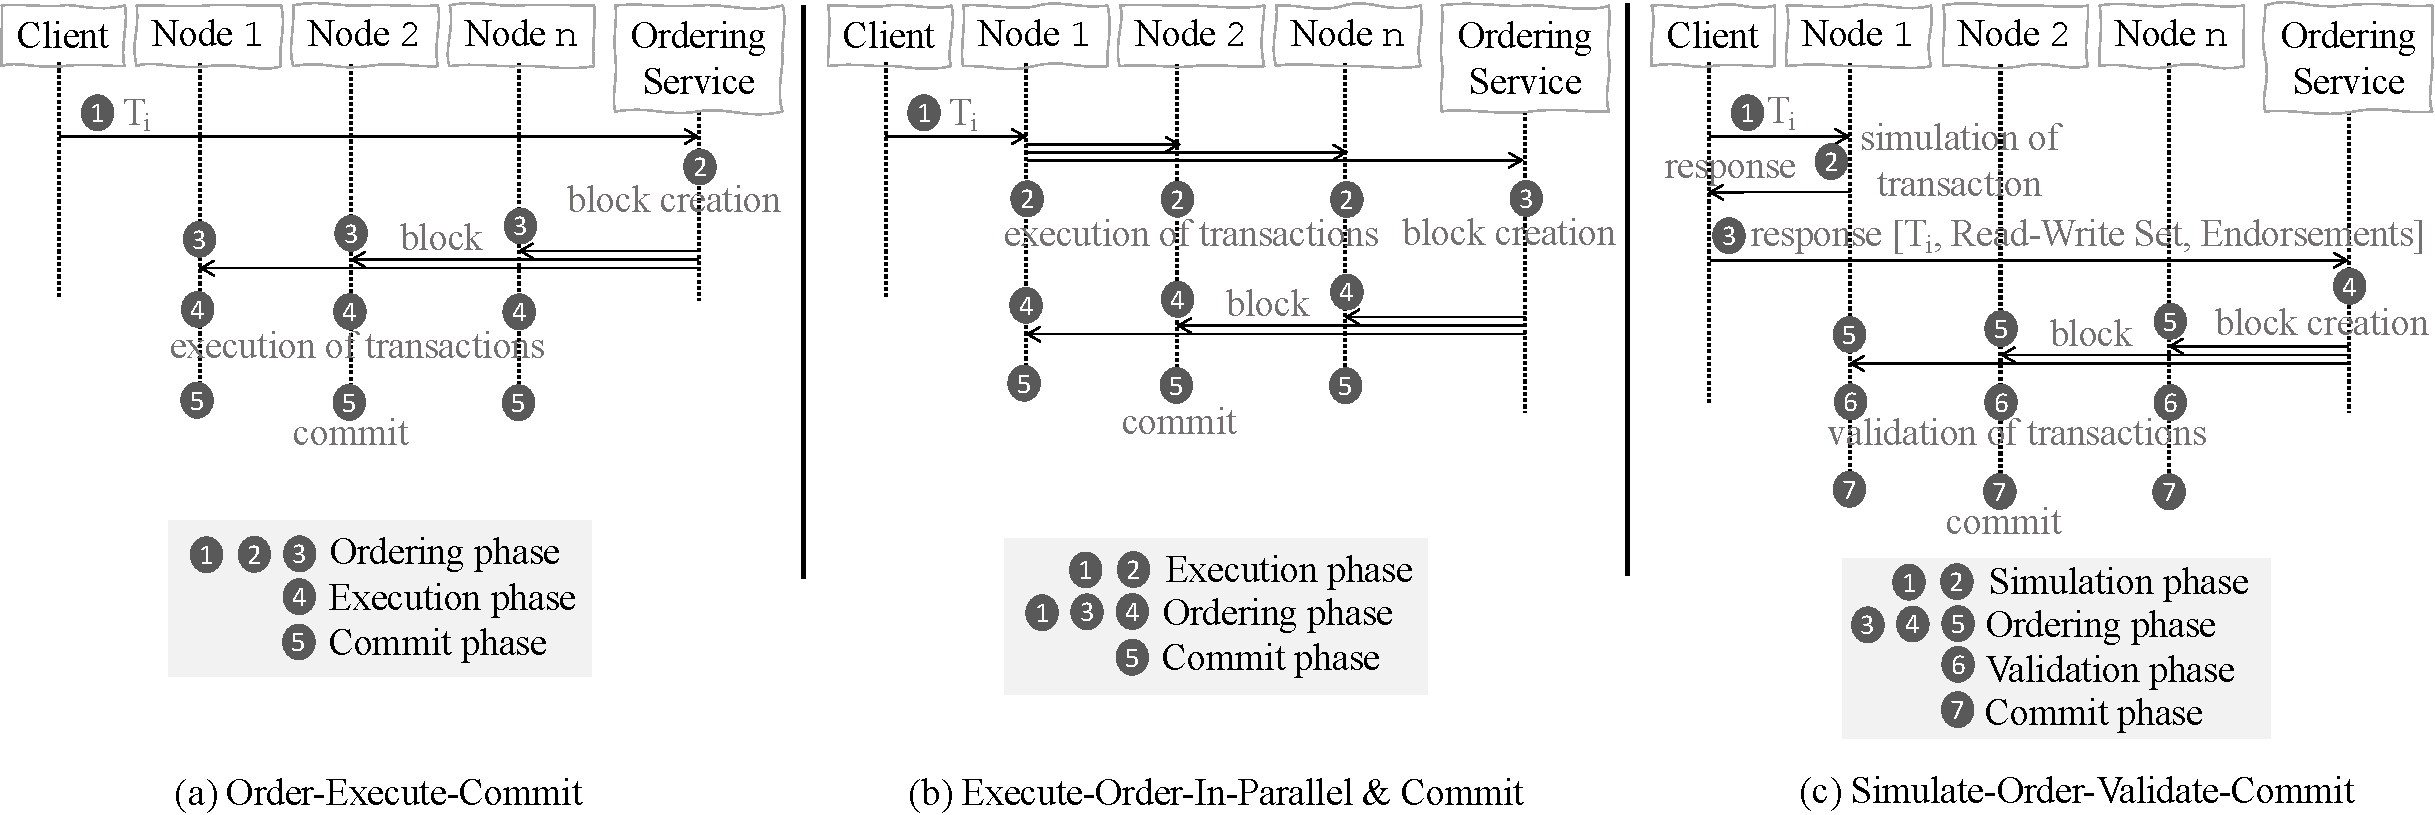
\includegraphics[scale=0.42]{fig/replication-protocol.pdf}
  		\vspace{-.4cm}
        \caption{\small{Blockchain replication protocols}.}
		\label{fig:replication-protocol}
 \end{center}
  \vspace{-.5cm}
\end{figure*}
\section{Implication of Blockchain Replication Protocols on Private Data Collections}
This section considers three existing blockchain replication protocols depicted in Figure~\ref{fig:replication-protocol}
and discusses whether the proposed private data collection can be implemented while satisfying the design requirements specified in 
% §3. 
% In this section, we consider three existing blockchain replication protocols depicited in 
% and discuss whether the proposed private data collection can be implemented while satisfying the design requirements
% specified in 
\S\ref{pdc}. %Note that it is possible to implement requirements R4 and R5 in all three
%existing replication protocols, and hence it is not discussed in this section
Note that in these replication protocols, the identifier or name of the smart-contract
that executes a transaction is specified in the transaction input itself along with the other inputs
required for the execution of contract functions.
\subsection{Order-Execute-Commit} 
\label{order-execute-commit}
Figure~\ref{fig:replication-protocol}(a) presents the three phases, (1) ordering, (2) execution, and (3) commit,
of this replication protocol. In the
ordering phase, first, the user-submitted transactions are ordered, and a block is generated through
mining/consensus. Second, the created block is broadcasted to all nodes in the blockchain network. In the
execution phase, on receiving a block, each node executes transactions present in the block serially by invoking the appropriate
smart-contract. Finally, in the commit phase, the executed transactions are committed.
Ethereum~\cite{}, Quorum~\cite{}, and Hyperledger Besu~\cite{} implement order-execute-commit replication protocol.
In this protocol, the transactions are passed to all nodes via a block. All nodes execute the transactions. Hence, it is not
trivial to support requirement R2 listed in \S\ref{pdc}.
% In this replication protocol, first, the user-submitted transactions are ordered, and a block is generated through
% mining/consensus. Second, the created block is broadcasted to all nodes in the blockchain network. Third, on receiving
% a block, each node executes the transaction serially by invoking the appropriate smart-contract and commit the same.
% Ethereum~\cite{}, Quorum~\cite{}, and Hyperledger Besu~\cite{} implements order-execute-commit replication protocol.
% In this protocol, the transaction input are passed to all nodes via a block. All nodes execute the smart-contract
% using the input. Hence, it is not possible to support requirement R1 listed in \S\ref{pdc} with this protocol.
% Given that transaction input go to all nodes, we need to pass the private data to members' node via
% a separate mechanism and only pass the hashed state in the transaction input. However, with this solution, it
% is not possible to support requirements R1, R2, and R3 listed in \S\ref{pdc}. The requirement R1 cannot be satisfied
% because the smart-contract is executed on all nodes, i.e., even on the nodes which do not have access to the required
% private data collection.
% The requirement R2 cannot be satisfied as we need to store the private data separately before or after storing the hash
% on the replicated ledger using the smart-contract.
% The requirement R3 cannot be satisfied because the user cannot pass the pointer to the private
% data, such as order ID, in the transaction input that needs to be modified as it would reveal some information
% about the private data.
% Given these drawbacks, we decide not to pick the blockchain platforms
% which support only the order-execute-commit replication protocol.
\subsection{Execute-Order-In-Parallel \& Commit}
Figure~\ref{fig:replication-protocol}(b) presents the three phases, (1) execution, (2) ordering, and (3) commit,
of this replication protocol.
In the execution phase, submitted transactions are executed in parallel on nodes without prior knowledge of order,
while the ordering phase happens simultaneously through a consensus service or mining. Once the block is created and
delivered to nodes, the executed transactions would get committed/aborted depending on the commit phase's serializability
check. The BlockchainRDBMS~\cite{} implements this replication protocol. Similar to the order-execute-commit protocol,
it is not trivial to satisfy requirements R2.
% In the execution phase, submitted transactions are executed in parallel on nodes without prior knowledge of ordering
% while ordering phase happens simultaneously through a consensus service or mining. Once the block is created and
% delivered to nodes, the executed transactions would get committed/aborted depending on the serializability check
% in the commit phase.
% If a node never received a transaction that is present in the block, it would execute the transaction and commit.
% The BlockchainRDBMS~\cite{} implements this replication protocol. Similar to the
% order-execute-commit protocol, it is not trivial to satisfy requirements R2.
\subsection{Execute-Order-Validate-Commit.}
Figure~\ref{fig:replication-protocol}(c) presents the four phases, (1) execution, (2) ordering, (3) validation, and
(4) commit, of this replication protocol.
In the execution phase, the transaction is executed on a sub-set
of nodes depending on the endorsement policy defined for a smart-contract. As a result of transaction execution,
the read-write set is collected. In the ordering phase, the read-write set and
endorsements are sent to the consensus service for transaction ordering and block creation. Once the block is created,
it is delivered to all nodes in the blockchain network. In the validation phase, on receiving the block, each node verifies whether
the transaction has collected enough endorsements as per the policy defined for the invoked smart-contract and executes
Optimistic Concurrency Control~\cite{} using the read-write set to perform serializability check. Finally, in the commit phase,
only valid serializable transactions are committed. Hyperledger Fabric~\cite{} implements execute-order-validate-commit
replication protocol.
% \par
We can implement private data collection with this replication protocol while satisfying all six requirements
mentioned in \S\ref{pdc} as shown in \S\ref{}.
% To satisfy requirement R1 and R2, we can pass the private data in the transaction input itself
% and simulate the transaction only on nodes which are the members of the private data collection. To ensure that
% only members stores the private data, during transaction simulation, we can store the private data in a temporary store
% and include only the hash of private data in the read-write set which goes to all nodes via a block for validation
% and commit. During commit, for valid transactions, we can fetch the corresponding private data from the temporary store.
% Thus, the requirements R3 and R4 are satisfied. The other requirements can also be satisfied as shown in \S\ref{}.
% Given that transaction can be simulated on a sub-set of nodes, we can pass the private
% data in the transaction input itself and simulate the transaction as per the collection membership. Thus, the
% smart-contract can access both private and public states which satisfies the requirement R1. As the simulation
% result includes read-write set, we can make the node to compute and store only the hash of private data in the
% read-write set which goes to all node to get stored in the replicated ledger. During transaction simulation,
% we can store the private data in a temporary store and fetch it while processing the read-write set during the
% commit time. Thus, we can satisfy requirements R2 and R3.


% \section{Design of Public Ledger}
some text \ldots

\subsection{Channels and Pluggable Database Layer}
some text \ldots

\subsection{Transaction Simulation, Validation, and Commit}
some text \ldots

\subsection{Block Storage}
some text \ldots

\subsection{History Database and Provenance Queries}
some text \ldots

\subsection{Failure and Recovery}
some text \ldots

\subsection{Point in Time Rollback}
some text \ldots

\subsection{Backup and Restore}
some text \ldots


\section{Design of Private Ledger}
some text \ldots

\subsection{Private Data Collection}
some text \ldots

\subsection{Transaction Simulation, Validation, and Commit}
some text \ldots

\subsection{Private Data Store}
some text \ldots

\subsection{Missing Private Data, Dynamic Collection, and Reconciliation}
some text \ldots

\subsection{Purging of Expired Private Data}
some text \ldots

\subsection{Failure and Recovery}
some text \ldots

\subsection{Point in Time Rollback}
some text \ldots




\section{Private Data Dissemination and Retrieval}
\label{s:gossip}
Since private data is excluded from the consensus-driven block delivery, we utilize a specialized peer-to-peer protocol to ensure data availability and fault tolerance. The protocol operates in two complementary phases: proactive dissemination during simulation, and reactive retrieval during commit.

\subsection{Proactive Dissemination}
\label{s:dissemination}
During the simulation phase, each endorsing node stores the generated private write-sets in its local transient store and proactively pushes them to a subset of authorized remote peers via a peer-to-peer protocol. For each collection involved in the transaction, the endorser sends the entire collection's private write-set as a single message to eligible peers. The set of target peers is determined by evaluating the collection's membership policy $\mathcal{M}$ against the current view of active peers in the network. The number of peers targeted is governed by $n_{dissem}$, and the endorser waits until at least $n_{required}$ peers acknowledge receipt before returning the signed endorsement response to the client. This eager strategy ensures that the private data is already present on most authorized nodes by the time the corresponding block is received, minimizing the need for reactive pulling during the commit phase. If the endorser cannot obtain $n_{required}$ acknowledgments before the timeout, it returns a dissemination failure to the client; the client may then retry with a different set of endorsers or abort the transaction. The endorser itself does not re-attempt dissemination, as the client is responsible for orchestrating retries---this keeps the endorser stateless with respect to dissemination attempts. Algorithm~\ref{alg:dissemination} summarizes the protocol.

\begin{algorithm}[h]
\centering
\small
\begin{tabular}{|p{0.92\columnwidth}|}
\hline
\textbf{Proactive Dissemination Protocol} \\
\hline
\textbf{Input:} Transaction $tx$ with private write-sets \\[3pt]
\textbf{At Endorsing Node} $e$ (after simulation): \\
\quad 1. Store all private write-sets for $tx$ in local transient store \\
\quad 2. \textbf{for each} collection $c$ in $tx$'s private write-sets \textbf{do} \\
\quad\quad\quad $W_c \leftarrow$ collection $c$'s private write-set \\
\quad\quad\quad $P \leftarrow \text{SelectAuthorizedPeers}(c.\mathcal{M}, c.n_{dissem})$ \\
\quad\quad\quad \textbf{for each} peer $p_i \in P$ \textbf{do} \\
\quad\quad\quad\quad\quad Push $(tx.id, c.id, W_c)$ to $p_i$ via gossip \\
\quad\quad\quad Wait until $|\{p_i : \text{ACK received}\}| \geq c.n_{required}$ \\
\quad\quad\quad\quad\quad or timeout expires \\
\quad\quad\quad \textbf{if} timeout \textbf{then} return dissemination failure \\
\quad 3. Return signed endorsement response to client \\[3pt]
\textbf{At Receiving Peer} $p_i$: \\
\quad 1. Verify sender $e$ is authorized for collection $c$ \\
\quad 2. Verify ledger height of $tx$ is within acceptable range \\
\quad 3. Store $(tx.id, c.id, W_c)$ in local transient store \\
\quad 4. Send ACK to endorser $e$ \\
\hline
\end{tabular}
\caption{Proactive dissemination protocol executed during the simulation phase. The endorser pushes each collection's full private write-set to authorized peers before returning the endorsement.}
\label{alg:dissemination}
\end{algorithm}


\subsection{Reactive Retrieval}
\label{s:retrieval}
Despite hash pre-images can be disseminated to target peers before they receive the block that contains the corresponding hashes, a robust solution is needed with withstand network partitions and peer crashes which prevent the hash pre-images from reaching all the required peers. Furthermore, if new peers are added to the Blockchain, they can only obtain the required pre-images by pulling them from peers that posses them.

To that end, prior to committing a block to the ledger, a peer iterates through all hashed key writes in all transactions of the Block and analyzes whether it needs to pull private data for each hashes key write. A hashed key write is considered as a viable candidate for pulling pre-images if:
\begin{itemize}
	\item The transaction passed validation of endorsement policies {Are we into abstracting out EPs? If yes then how should I phrase this?}. This is needed in order to prevent a denial-of-service attack in which a malicious party creates  transactions with hashed writes for which there are no pre-image in any peer in the network. Peers would try to pull these transactions and fail, hence considerably slowing down throughput.
	\item Evaluation of the collection policy on the peer's identity returns "true" {Once we define collection policies more abstractly we need to change this as well}: this is required since peers that receive pre-image requests for a certain hashed write also evaluate the same collection policy on the requester peer's identity in order to determine if that peer is part of the collection the hashed write is associated with.
	\item Whether the peer is missing the pre-image from its transient store, since by definition this means the pre-image hasn't been disseminated to the peer before the commit of the block.
	\item {Should we mention purged private data?}
\end{itemize}

Once the peer decides it needs to pull a hashed write, it needs to select potential peers which might have the pre-image it needs, and send them requests for the digests.
Upon reception of responses containing pre-images, the peer validates that the hashes on the pre-images received matches the hashed write in the block. It follows from the collision resistance property of the cryptographic hash function that if the responding peer sent a pre-image of a hashed write, then with overwhelming probability, the pre-image is identical to all pre-images in all peers in the network, hence consistency is preserved.

When sending requests for pre-images, a requester peer doesn't know up-front whether the responder peer has the pre-image, and every such "wrong guess" results in a retry which delays the block commit and thus hinders performance.

For this reason, the peers prioritize requesting a pre-image from the peers which endorsed the transaction {This is very Fabric specific, so we might want to remove this?} from which the hashed write originated. This is possible because peers constantly maintain a membership view of alive peers by periodically disseminating heartbeats. 



\subsection{Dynamic Membership and Reconciliation}
\label{s:dynamic-membership}
Collection membership may change over the lifetime of a network. When a new member is added to a collection's membership policy $\mathcal{M}$, the peer detects the configuration change during the commit of the block containing the policy update and initiates a retroactive reconciliation process. Specifically, the peer scans the committed blocks for historical transactions that wrote to the collection and marks them as missing eligible data. A background reconciliation service then periodically pulls these historical private write-sets from existing collection members using the same hash-based verification as the reactive retrieval protocol.

When a member is removed from a collection, the removed peer retains access only to data committed before its removal. The updated membership policy excludes it from both proactive dissemination and reactive retrieval eligibility checks, ensuring that future private data is not shared with the departing organization.

\subsection{Consistency and Fault Tolerance}
A critical property of the retrieval mechanism is its idempotency: since multiple peers may attempt to pull the same missing data concurrently, the system utilizes the versioned hashes on the public ledger as unique identifiers, ensuring that nodes eventually converge on a consistent Private State even in the presence of network partitions or concurrent block commits.

\smallskip
\noindent\textbf{Remark} (Integrity Independence). \textit{Data integrity is preserved even when peers attempt to provide fraudulent pre-images, because the requester validates every incoming data piece against the on-chain hash recorded during the consensus phase. This integrity guarantee operates independently of the CFT assumption described in \S\ref{pdc}: while the \textbf{liveness} of dissemination depends on honest peers following the protocol, the \textbf{correctness} of retrieved data is ensured solely by cryptographic hash verification. A single honest data source is sufficient for correctness.}



% \section{Design of Gossip Protocol}
very tentative. just to put out a layout.

\subsection{Membership Information}
some text \ldots

\subsection{Block Dissemination and Channels}
some text \ldots

\subsection{Private Data Dissemination During Simulation and Commit}
some text \ldots

\subsection{Reconciliation of Missing Private Data}
some text \ldots

\subsection{Block Reprocessing After a Rollback}
some text \ldots


\section{Threat Model and Security Analysis}
\label{s:threat-model}
Our design assumes a decentralized network of organizations where a subset of nodes may be faulty or malicious. We describe the trust assumptions for each entity and analyze the security implications when these assumptions are violated.

\textit{Peer Nodes.} We assume a crash-fault tolerant (CFT) model for authorized peers. A malicious peer may attempt to (a)~leak private data it is authorized to see, or (b)~refuse to disseminate data, but a single compromised peer cannot manipulate the ledger state because the integrity of the public ledger is protected by the endorsement policy, which requires signatures from multiple organizations before a transaction is considered valid. Data manipulation is only possible if a majority of the endorsing organizations collude. \textit{Correctness} is preserved as long as the endorsement policy holds---that is, a sufficient number of endorsing organizations remain honest. If a majority of the endorsing organizations collude, they can endorse fraudulent transactions with manipulated hashes, compromising both the private data and the on-chain evidence. Data \textit{confidentiality} within a collection is bounded by the weakest member---a compromised member can exfiltrate any private data it is authorized to access. \textbf{This is an inherent limitation of any access-control-based (as opposed to cryptographic) privacy mechanism}: the system ensures that unauthorized parties never receive private data, but it cannot prevent an authorized party from misusing data it legitimately possesses. Organizations mitigate this risk through legal agreements, hardware security modules, and operational controls.

\textit{Ordering Service.} The ordering service is a decentralized cluster operated by consortium organizations---potentially the same organizations that run peers. Its role is strictly limited to establishing the total order of transactions; it never sees private data payloads, as only public and hashed read-write sets are submitted for ordering. Standard BFT security assumptions apply: as long as fewer than one-third of the ordering nodes are Byzantine, the ordering service guarantees liveness and correct ordering.

\textit{Clients.} Clients may be malicious, attempting to submit inconsistent private data to different endorsers or forge simulation results. If a client sends different private data to different endorsers, each endorser will compute a different hash of the private data and include it in its signed endorsement response. Since the endorsement policy requires matching responses from multiple endorsers, the inconsistent hashes will cause the endorsements to be incompatible, and the transaction will be rejected during validation. A malicious client may also simulate many transactions but never submit them to the ordering service, leading to the accumulation of orphan write-sets in the transient store. To mitigate this, we introduce a retention window $\Delta$: the transient store automatically purges any entries where the current ledger height exceeds the simulation height by more than $\Delta$. Receiving peers also reject disseminated write-sets outside this window. A second attack vector involves fabricated simulations lacking sufficient endorsements; to counter this, peers perform endorsement policy validation \emph{before} attempting to pull any missing pre-images, skipping invalid transactions entirely.

\textit{Network.} We assume a partially synchronous network where partitions are possible but eventually resolve, allowing for asynchronous data reconciliation. During a partition, private data dissemination may be delayed but the system does not compromise correctness---peers that cannot obtain private data before commit track it as missing and reconcile asynchronously once connectivity is restored.



\section{Implementation}
some text \ldots


\section{Evaluation}

\textbf{TODO: Evaluation experiments to include:}
\begin{enumerate}[topsep=0pt,noitemsep,leftmargin=15pt]
    \item Throughput comparison: PDC transactions vs.\ standard transactions
    \item Latency breakdown across the four phases (simulation, ordering, validation, commit)
    \item Scalability with number of collections, organizations, and private data sizes
    \item Gossip overhead: network bandwidth for dissemination and retrieval
    \item Impact of block-to-live (purging) on performance
    \item Comparison with channel-based isolation (the main alternative)
    \item Failure/recovery scenarios and their performance impact
    \item Addition of new members to the collection and sync/fetch duration
\end{enumerate}


\section{Real-World Impact}

Since its introduction in Hyperledger Fabric v1.2, the private data collection mechanism has seen significant adoption across diverse industries. In mining and metals, MineHub~\cite{minehub} explicitly credits PDCs for enabling their supply-chain platform to scale to thousands of companies, replacing the coarse-grained channel model that could not support their dynamic data-sharing requirements. In food safety, the IBM Food Trust---deployed at Walmart and other major retailers~\cite{walmart-hf}---leverages PDCs to protect supplier-specific data such as pricing and proprietary process steps while maintaining end-to-end traceability. In global trade, GSBN (Global Shipping Business Network)~\cite{gsbn} uses PDCs for private trade documents such as Bills of Lading across its permissioned shipping network. In pharmaceuticals, the MediLedger project~\cite{mediledger} combines PDCs with zero-knowledge proofs to achieve even higher levels of privacy for drug tracking under the U.S. Drug Supply Chain Security Act (DSCSA), as validated by an FDA pilot program. These deployments demonstrate that private data collections address a genuine enterprise need and that the design choices described in this paper---particularly the balance between on-chain verifiability and off-chain confidentiality---translate effectively to production environments.


\section{Related Work}
\yacov{I'll take this part if you don't mind $:)$}
\textbf{(1) Fabric Channel.}
\par
\textbf{(2) Quorum~\cite{} Private Transaction.}
\par
\textbf{(3) Encryption of Data.}
\par
\textbf{(4) Zero Knowledge Proof.}



\section{Conclusion}

We presented \textit{private data collections} (PDCs): private data is stored only on authorized peers while its cryptographic hash is recorded on the replicated ledger. The key theoretical result is that on-chain hashes form a \textit{conflict-complete proxy} for private state (Theorem~1): optimistic concurrency control (OCC)~\cite{occ} based serializability checks on hashed state detect exactly the same conflicts as checks on the underlying private data, enabling network-wide correctness verification without accessing private data. A transient store, hashed read-write sets, and a three-component dissemination protocol deliver privacy, atomicity, integrity, and auditability within a single shared ledger---without specialized hardware, expensive cryptographic primitives, or channel-based overhead. Our Hyperledger Fabric implementation, production-ready since v1.2, adds 3--14\% overhead. Deployments at Walmart, MediLedger, GSBN, and MineHub confirm cross-industry generality.


% The following two commands are all you need in the
% initial runs of your .tex file to
% produce the bibliography for the citations in your paper.
\balance
\bibliographystyle{abbrv}
\bibliography{paper}  % vldb_sample.bib is the name of the Bibliography in this case
% You must have a proper ".bib" file
%  and remember to run:
% latex bibtex latex latex
% to resolve all references

\end{document}
%%% Local Variables:
%%% mode: latex
%%% TeX-master: t
%%% End:
